% Created 2024-05-08 Wed 00:23
% Intended LaTeX compiler: pdflatex
\documentclass[11pt]{article}
\usepackage[utf8]{inputenc}
\usepackage[T1]{fontenc}
\usepackage{graphicx}
\usepackage{longtable}
\usepackage{wrapfig}
\usepackage{rotating}
\usepackage[normalem]{ulem}
\usepackage{amsmath}
\usepackage{amssymb}
\usepackage{capt-of}
\usepackage{hyperref}
\author{Kritika Prasai}
\date{\today}
\title{}
\hypersetup{
 pdfauthor={Kritika Prasai},
 pdftitle={},
 pdfkeywords={},
 pdfsubject={},
 pdfcreator={Emacs 28.1 (Org mode 9.5.2)}, 
 pdflang={English}}
\begin{document}

\tableofcontents

\section{Project Title:MINDSTREAM: Decoding Brain Signals into Text with NLP}
\label{sec:orgd3539bf}

\section{Table of contents}
\label{sec:org9bd2a98}
\subsection{Abstract}
\label{sec:org3f6a85a}
\subsection{Introduction}
\label{sec:org185744e}
\subsection{Dataset Description}
\label{sec:org281a632}
\begin{itemize}
\item Dataset details
\item Pre-processing
\end{itemize}
\subsection{Literature Review}
\label{sec:orgebfc69c}
\subsection{Methods and Materials}
\label{sec:org8f4d832}
\begin{itemize}
\item Model pipeline
\item Model Architecture
\item Implementation Details
\item Results and Evaluation
\end{itemize}
\subsection{Challenges}
\label{sec:orgbb63d8e}
\subsection{Conclusion}
\label{sec:org1f0db80}
\begin{itemize}
\item Future Works
\end{itemize}
\subsection{Code Description}
\label{sec:orga8ff932}
\subsection{Refrences}
\label{sec:org9a689b4}

Abstract:
\begin{justify}
Brain-Computer Interfacing (BCI) holds immense potential for revolutionizing human-computer interaction by directly translating brain activity into actionable commands. In this project, we explore the application of BCI technology in the realm of natural language processing (NLP) through the analysis of electroencephalography (EEG) data. Leveraging the ZuCo dataset, we investigate the feasibility of decoding EEG signals into textual representations and further extend our analysis to sentiment classification tasks.

Our methodology involves the utilization of deep learning models to process EEG signals and extract meaningful features for downstream NLP tasks. We employ state-of-the-art pre-trained models for embeddings to enhance the representational power of our EEG data. Through rigorous experimentation and evaluation, we assess the performance of various deep learning architectures in transforming EEG data into textual and sentiment-related information.

The results of our study demonstrate the potential of BCI technology in bridging the gap between neural signals and natural language, showcasing promising capabilities in tasks such as EEG-to-text translation and sentiment analysis. Our findings contribute to the growing body of research in BCI applications and highlight avenues for future exploration in the intersection of neuroscience and natural language processing.Your paragraph text here. You can write multiple lines and they will all be justified aligned.
\end{justify}


\begin{enumerate}
\item Introduction:
\end{enumerate}
\begin{justify}
Our project "MINDSTREAM: Decoding Brain Signals into Text with NLP" explores the intriguing intersection of brain-computer interfacing (BCI) and natural language processing (NLP). While BCI technology has made remarkable strides in restoring motor functionalities for individuals with disabilities through motor imagery, decoding natural language directly from brain signals remains a formidable challenge. Previous approaches have encountered limitations in vocabulary size, device dependency, and articulation variability.This project extends the scope of BCI applications by transitioning from closed to open vocabulary EEG-to-text sequence-to-sequence decoding and zero-shot sentiment classification. Leveraging the ZuCo dataset and non-invasive EEG recordings, in this study we work on using deep learning models and pre-trained language embeddings to capture complex linguistic information from brain signals.

Inspired by recent advancements in large-scale pretrained language models such as BERT and GPT, the project explores the transfer learning capabilities of these models for EEG-to-text decoding. By fine-tuning pretrained language models and additional projection layers, the study aims to unlock contextualized representations of brain signals, encompassing syntactic and semantic features.

Moreover, the project underscores the importance of non-invasive EEG data due to its high temporal resolution and accessibility. While invasive devices like ECoG may offer superior performance, EEG provides a cost-effective and readily available alternative, crucial for training data-hungry models. Most importantly, this project aims at introducing novel tasks in open vocabulary EEG decoding and EEG-based sentiment classification taking inspirations from existing literatures and explores about how we are  marking towards a significant step forward in BCI-NLP integration. Integrating the  pretrained language models and non-invasive EEG data, we try to shed some light on the potential of BCI technology as a transformative tool for human-machine interaction in diverse domains.

\end{justify}

\begin{enumerate}
\item Dataset:
\end{enumerate}
2.1 What is EEG signals?
\begin{justify}
EEG (Electroencephalography) signals are recordings of electrical activity generated by the brain, measured by placing electrodes on the scalp. These signals reflect the synchronized activity of large groups of neurons and are widely used in neuroscience to study brain function in various cognitive processes.
\end{justify}

\begin{center}
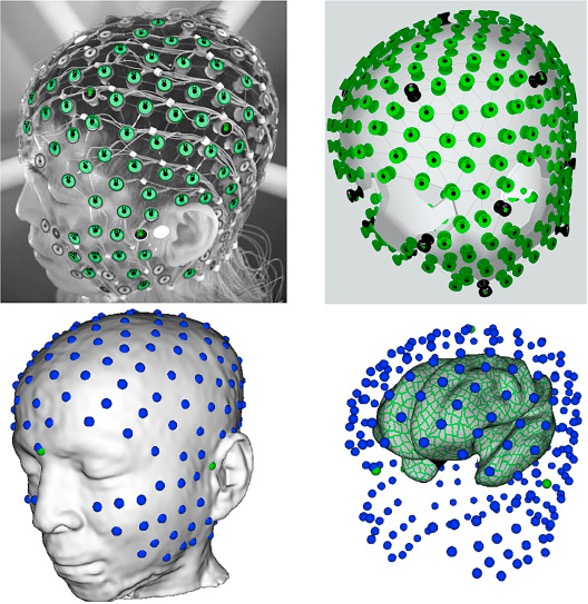
\includegraphics[width=.9\linewidth]{../Figures/EEG_data_collection.jpg}
\end{center}

2.2 Understanding how brain works during reading or thinking: Simplifying Brain Processes
\begin{justify}
When it comes to reading and thinking, EEG provides valuable insights into the underlying neural mechanisms. During reading, specific patterns of brain activity emerge, reflecting the processing of visual information, language comprehension, and memory retrieval. Different stages of reading, such as word recognition, semantic processing, and comprehension, are associated with distinct EEG signatures. Similarly, during thinking or cognitive tasks, EEG reveals patterns of neural synchronization and oscillatory activity across different brain regions. Mental processes involved in reading and thinking, such as attention, working memory, and executive functions, can be inferred from EEG signals. By analyzing these EEG patterns, researchers can gain a deeper understanding of how the brain processes information during reading and thinking tasks, shedding light on cognition and its underlying neural basis.
\end{justify}

\begin{center}
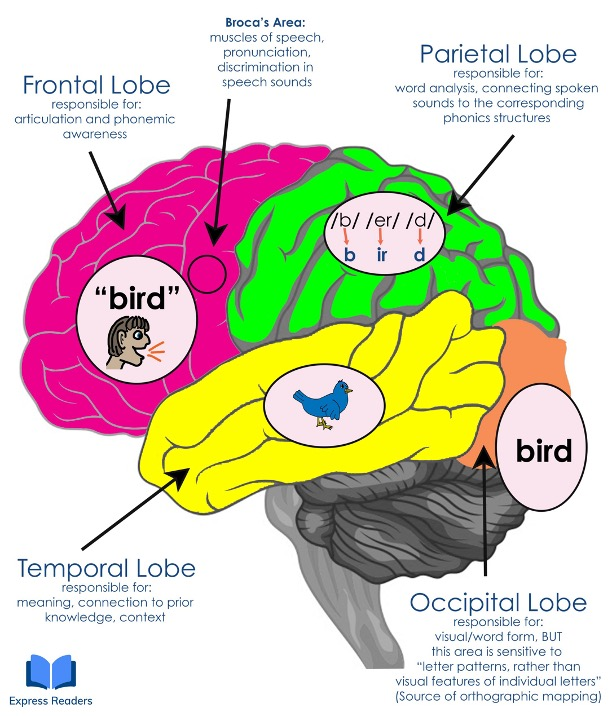
\includegraphics[width=.9\linewidth]{../Figures/Brain_signals.jpg}
\end{center}

\section{Attention: The ability to focus on specific stimuli while ignoring others. beta waves (13-30 Hz) and gamma waves (30-100 Hz) in the frontal and parietal lobes.}
\label{sec:orgc587858}
\section{Memory: The process of encoding, storing, and retrieving information. Differences in theta waves (4-7 Hz) and gamma waves during encoding and retrieval processes.}
\label{sec:org858761a}
\section{Language comprehension: The ability to understand and interpret language. Semantic processing (e.g., N400 component) and syntactic processing (e.g., P600 component)}
\label{sec:org95c0e49}

\begin{center}
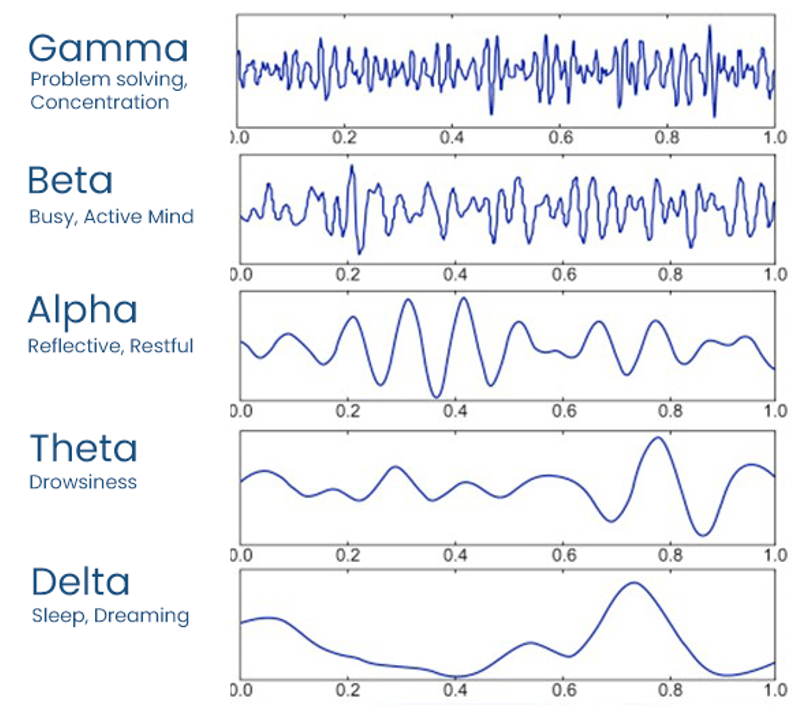
\includegraphics[width=.9\linewidth]{../Figures/EEG_signals.png}
\end{center}

2.3 Decoding EEG to text and its importance:
\#+BEGIN\textsubscript{EXPORT} latex
\begin{justify}
\section{Communication for disabled individuals: such as locked-in syndrome or severe motor disabilities, to express themselves through text.}
\label{sec:org3ff4cea}
\section{Brain-computer interfaces (BCIs): BCIs can enable control of computers, prosthetic devices, and other technologies using only brain activity.}
\label{sec:org1940066}
\section{Understanding brain function: can provide valuable insights into the neural mechanisms underlying language production and comprehension.}
\label{sec:org829e6ec}
\section{Medical applications: EEG-based text decoding can aid in diagnosing and monitoring neurological disorders such as epilepsy, sleep disorders, and cognitive impairments.}
\label{sec:orgb9fc26c}
\section{Assistive technology: Decoding EEG to text can be used to develop assistive technologies that enhance communication and quality of life for individuals with disabilities.}
\label{sec:orgba9dc8e}
\end{justify}
\#+END\textsubscript{EXPORT}   

2.4 Zuco Dataset Description:
\begin{justify}
The Zurich Cognitive Language Processing Corpus (ZuCo) is a valuable resource for studying language processing, incorporating simultaneous eye-tracking and electroencephalography (EEG) data during natural reading and linguistic annotation tasks. ZuCo 2.0, introduced in the paper "ZuCo 2.0: A dataset of simultaneous EEG and eye-tracking recordings during natural reading" by P. Lüdtke et al., expands upon its predecessor, ZuCo 1.0, with additional data and improved methodologies. Comprising 739 sentences, ZuCo 2.0 includes 349 sentences from standard reading paradigms and 390 from task-specific linguistic annotation tasks. These tasks involve participants actively seeking specific semantic relations within sentences. The dataset provides comprehensive insights into cognitive processes during language comprehension, offering researchers a rich resource to explore the neural correlates of reading and linguistic processing. Moreover, ZuCo 2.0 complements ZuCo 1.0 by enhancing the breadth and depth of available data, facilitating more robust analyses and discoveries in the field of cognitive neuroscience and natural language processing. The zuco dataset can be downloaded from below link 
\end{justify}
\url{https://osf.io/2urht/wiki/home/}

2.4.1 Data Preprocessing: Eye Tracking

\section{Data Acquisition: Eye position and pupil size were recorded using an EyeLink 1000 Plus tracker at 500 Hz.}
\label{sec:org0b190b2}
\section{Calibration: The eye tracker was calibrated with a 9-point grid before each paradigm, ensuring accuracy of gaze data.}
\label{sec:orge0bc316}
\section{Preprocessing:}
\label{sec:org789d466}
Saccades were detected based on velocity and acceleration thresholds.
Fixations were defined as periods without saccades.
Blinks were identified as periods with zero pupil diameter or zero gaze positions.
Fixations within the boundaries of each displayed word were extracted for analysis.
\section{Feature Extraction:}
\label{sec:orga713bbb}
Gaze duration (GD), total reading time (TRT), first fixation duration (FFD), single fixation duration (SFD), and go-past time (GPT) were extracted for each word.
Pupil size was computed for each of these eye-tracking features.
Number of fixations and mean pupil size were extracted for each word and sentence.
\section{Gaussian Mixture Model:}
\label{sec:orgd740d3b}
A Gaussian mixture model was trained on gaze data for each sentence to improve allocation of fixations to text lines.
Exclusion Criteria: Fixations shorter than 100 ms were excluded from the analyses, as they are unlikely to be relevant for reading.

2.4.2 Data Pre-processing: EEG data

\section{Data Acquisition: EEG data were recorded using 105 scalp electrodes and 9 EOG channels.}
\label{sec:org789ad45}
\section{Preprocessing Steps:}
\label{sec:orgb4504db}
EEG data were imported into MATLAB and triggers/latencies were extracted.
Bad electrodes were identified and replaced based on the EEGLab plugin clean\textsubscript{rawdata}.
EEG data were high-pass filtered at 0.5 Hz and notch filtered at 49-51 Hz.
Eye artifacts were removed by regressing EOG channels from scalp EEG channels.
MARA algorithm was used for automatic artifact rejection.
Bad electrodes were interpolated using spherical spline interpolation.
EEG and eye-tracking data were synchronized.
\section{Frequency Band Analysis:}
\label{sec:org27acc18}
Band-pass filtering was applied to extract data for five frequency bands.
Hilbert transform was used to compute the amplitude of each frequency band.
\section{Feature Extraction:}
\label{sec:org4db85b9}
EEG features were extracted based on sentence-level and fixation-based time segments from eye-tracking data.
Artifact Rejection:Trials with transient noise exceeding 90μV were excluded.

\begin{enumerate}
\item Literature Review:
\end{enumerate}


\begin{enumerate}
\item Methods and Materials:
\end{enumerate}

3.1 Model Pipeline:



3.2 Modification for Embedding Layer:


3.3 Implementation Details:

\section{Word embeddings play a crucial role in NLP tasks,  we use the BERT based transformer model to obtain token representations, which are then normalized using L2 normalization.}
\label{sec:orga0eec06}
\section{Each word is embedded into a 768-dimensional vector, resulting in a tensor of dimensions [N × M × 768], where N is the number of sentences and M is the maximum number of words per sentence.}
\label{sec:org5be34f9}
\section{To ensure consistency across sentences, padding is applied to handle variations in sentence length.}
\label{sec:org8695d5c}
\section{Eye-gaze features are extracted from the ZuCo dataset, encompassing 12 distinct features such as the Number of Fixations and Mean Pupil Size.}
\label{sec:org6050d6d}
\section{L1 normalization is applied to each eye-gaze feature within the sentence dimension to capture reading attention effectively.}
\label{sec:orgd179c52}
\section{For EEG data, the conditional entropy method is employed for feature extraction, resulting in a feature dimension of 5460.}
\label{sec:org997e4c8}
\section{Instances where no fixation occurs are assigned zero vectors, and for words with multiple fixations, the L2 norm is applied to each vector, followed by element-wise addition.}
\label{sec:orgfb11ee3}
\section{This comprehensive approach ensures a holistic representation of behavioral patterns in eye-gaze and EEG data.}
\label{sec:orgbac83c5}
\section{Instead of using concatenation, we project each feature into a shared space of 128 dimensions.}
\label{sec:org177353d}
\section{EEG and eye-gaze features are combined through element-wise addition.}
\label{sec:org616c637}
\section{After projection, sinusoidal positional encoding is applied before feeding the features into the transformer encoder.}
\label{sec:org5d9f301}
\section{Following the transformer encoder, a Multi-Layer Perceptron (MLP) is employed to predict the probabilities of input samples belonging to a specific label in this binary classification task.}
\label{sec:orge55a7f8}

3.4 Results and Evaluation:
\begin{figure}[htbp]
\centering
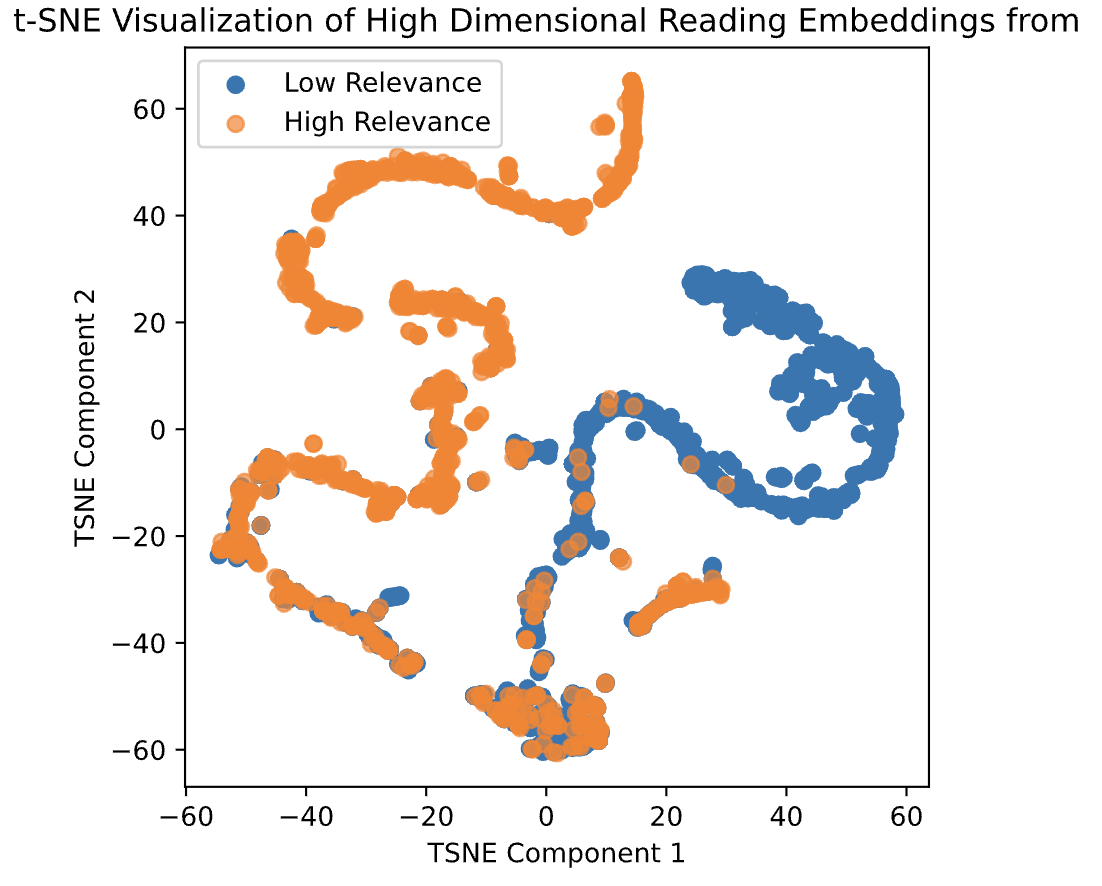
\includegraphics[width=.9\linewidth]{../Figures/Results_fig/Reading_embeddings.png}
\caption{show t-SNE visualizations showing the clustering of low- and high-relevance Reading Embeddings}
\end{figure}

\begin{figure}[htbp]
\centering
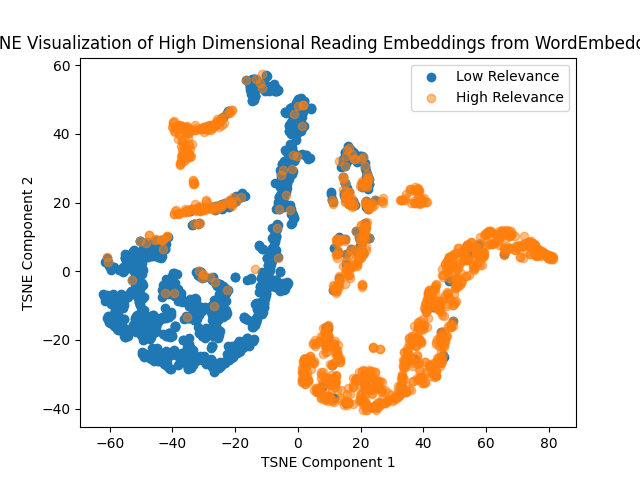
\includegraphics[width=.9\linewidth]{../Figures/Word_embeddings3.png}
\caption{show t-SNE visualizations showing the clustering of low- and high-relevance word  Embeddings}
\end{figure}
\end{document}